\section{Contour Integration of a Complex-valued Function}
\textit{(This problem is probably out of reach for students who not yet taken a course in complex analysis. No worries, we will cover this topic during the first few weeks of Math 583A.)}\\

\noindent Consider the functions $f:\mathbb{C} \to \mathbb{C}$ and $g:\mathbb{C} \to \mathbb{C}$ defined as
\begin{equation*}
f(z) = z^2 \quad \quad \text{and} \quad \quad g(z) = z^{-1}
\end{equation*}
In this project, you will write a first-order numerical approximation scheme to compare the integrals of $f$ and of $g$ along two different contours.
\begin{enumerate}[(a)]
    \item Plotting:
    \begin{enumerate}[i.] 
        \item Make a surface plot showing $Re(f(z))$ and a surface plot showing $Im(f(z))$
        \item Make a surface plot showing $Re(g(z))$ and a surface plot showing $Im(g(z))$
    \end{enumerate}
    \textit{Since $g$ is undefined at $z = 0$ and since it is radially symmetric, the surface plots for $g$ can look scary when done in cartesian co-ordinates. You may try switching to polar coordinates to make prettier plots}
    \item     We can approximate the line integral (or contour integral) of a function along a curve by discretizing the curve into $N+1$ points $z(s) \to \{z_0, z_1, z_2, \dots, z_N\}$ and then computing the sum:
    \begin{equation*}
    \int_{z_o}^{z_t} f(z) dz \approx \sum_{k = 1}^{N} f(z_k) \ (z_{k} - z_{k-1})
    \end{equation*}
    \begin{minipage}{.7\textwidth}
    Define the two curves:
    \begin{align*}
    C_1:&  \quad \text{The upper half circle of radius 1 centered at $z=0$.}\\
    C_2:&  \quad \text{The lower half circle of radius 1 centered at $z=0$.}
    \end{align*}
    Approximate the line integrals of $f$ and of $g$ along the curves $C_1$ and $C_2$.
    \end{minipage}
    \begin{minipage}{.29\textwidth}
    \begin{center}
    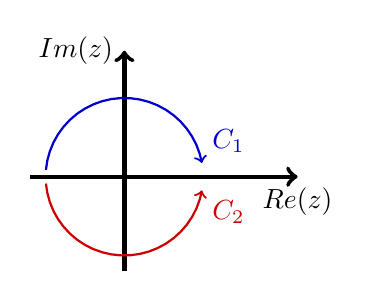
\begin{tikzpicture}
    \draw[ultra thick,->] (-1.2,0) -- (2.2, 0) node[below] {$Re(z)$};
    \draw[ultra thick,->] (0,-1.2) -- (0,1.6) node[left] {$Im(z)$};
    \draw[thick,blue!80!black,domain = 175:10,variable=\t,->] plot ({cos(\t)},{ sin(\t)}) node[above right] {$C_1$}; 
    \draw[thick,red!80!black,domain = 185:350,variable=\t,->] plot ({cos(\t)},{ sin(\t)}) node[below right] {$C_2$}; 
    \end{tikzpicture}
    \end{center}
    \end{minipage}
    \item[($\ast$)] \textit{Bonus:} Repeat parts (a) and (b) for the function $h(z) = z^{1/2}$.\\
    \textit{Note:} You may need to make some `executive decisions' to make sure your problem is well-posed.
\end{enumerate}

